\section{Expected Performance}
%- Rates\\
%- linearity \\
%- statistical precision

The performance of the Phase II OT has been studied using detailed detector simulations for a wide range of pile-up scenarios. The samples have been privately produced using CMSSW version 11\_2\_0\_pre6 and a custom geometry that includes only the tracker volume with geometry versions 6.1.3 and 6.1.6 for the Inner and Outer Tracker, respectively.They also contain simulated effects from front-end electronics, specifically for the OT 2S modules the CBC hit detection mode is set to latched. Similar to what was done for TEPX simulations (see section \ref{sec:TEPX_sim}), the process that has been used to generate these samples is a single-neutrino event overlaid with a variable number of minimum-bias events to simulate pile-up. 

To test the linearity, the number of stubs is histogrammed per event for each layer of the OT. The mean of these distributions is then plotted as a function of pile-up, and a line is fitted to the lowest pile-up points (between 0 and 2) and then extrapolated to higher values, up to a pile-up of 200. Figure \ref{fig:OT_linearity} shows the linearity of stubs for all OT barrel layers. The deviation from a perfectly linear behaviour is presented in figure \ref{fig:OT_deviation}, where it can be seen that layer 6 has a deviation of less than 1\% across the full pile-up range.

\begin{figure}[h!]
\centering
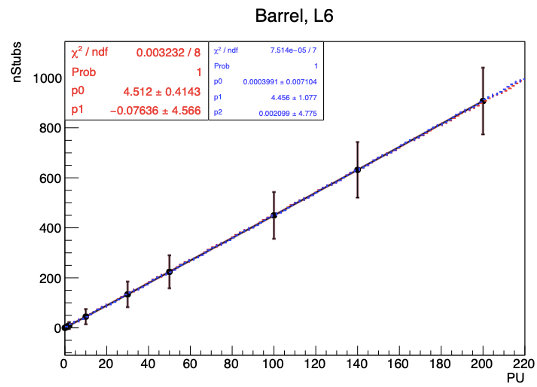
\includegraphics[width=.6\linewidth]{tex/Part2/fig/OT/OT-linearity.png}
\caption{
 Average number of track stubs per event as a function of pile-up determined from the CMS Phase II simulation showing a linear behaviour. \nts{PLACEHOLDER: To be replaced with a linearity plot including all barrel layers.}
} 
\label{fig:OT_linearity}
\end{figure}

\begin{figure}[h!]
\centering
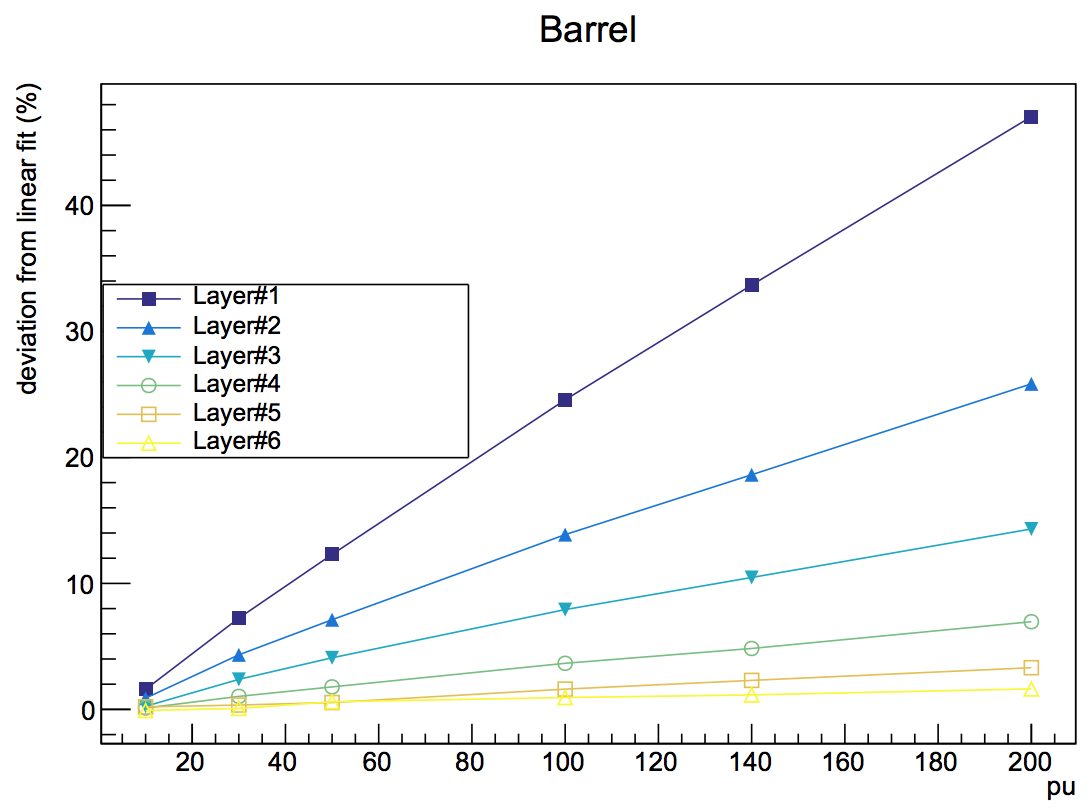
\includegraphics[width=.6\linewidth]{tex/Part2/fig/OT/OT-deviation.png}
\caption{
 Deviation from linearity for all barrel layers of the OT. \nts{PLACEHOLDER: To be replaced with plot using CMS style.}
}
\label{fig:OT_deviation}
\end{figure}

Another important figure of merit for the performance of the OT as a luminometer is the statistical precision that can be achieved. Figure \ref{fig:OT_rates} shows the average number of stubs per event per ladder in layer 6, obtained from the simulations described above. The maximum total rate for the pile-up step of 200 is found to be of 902 stubs per event for Physics and of 2.255 for vdM conditions. With these counts, and considering a trigger readout rate of 40~MHz and an integration period of 1~s (30~s), a statistical precision of 0.03\% (0.115\%) per bunch-crossing is expected for Physics (vdM) conditions.   

\begin{figure}[h!]
\centering
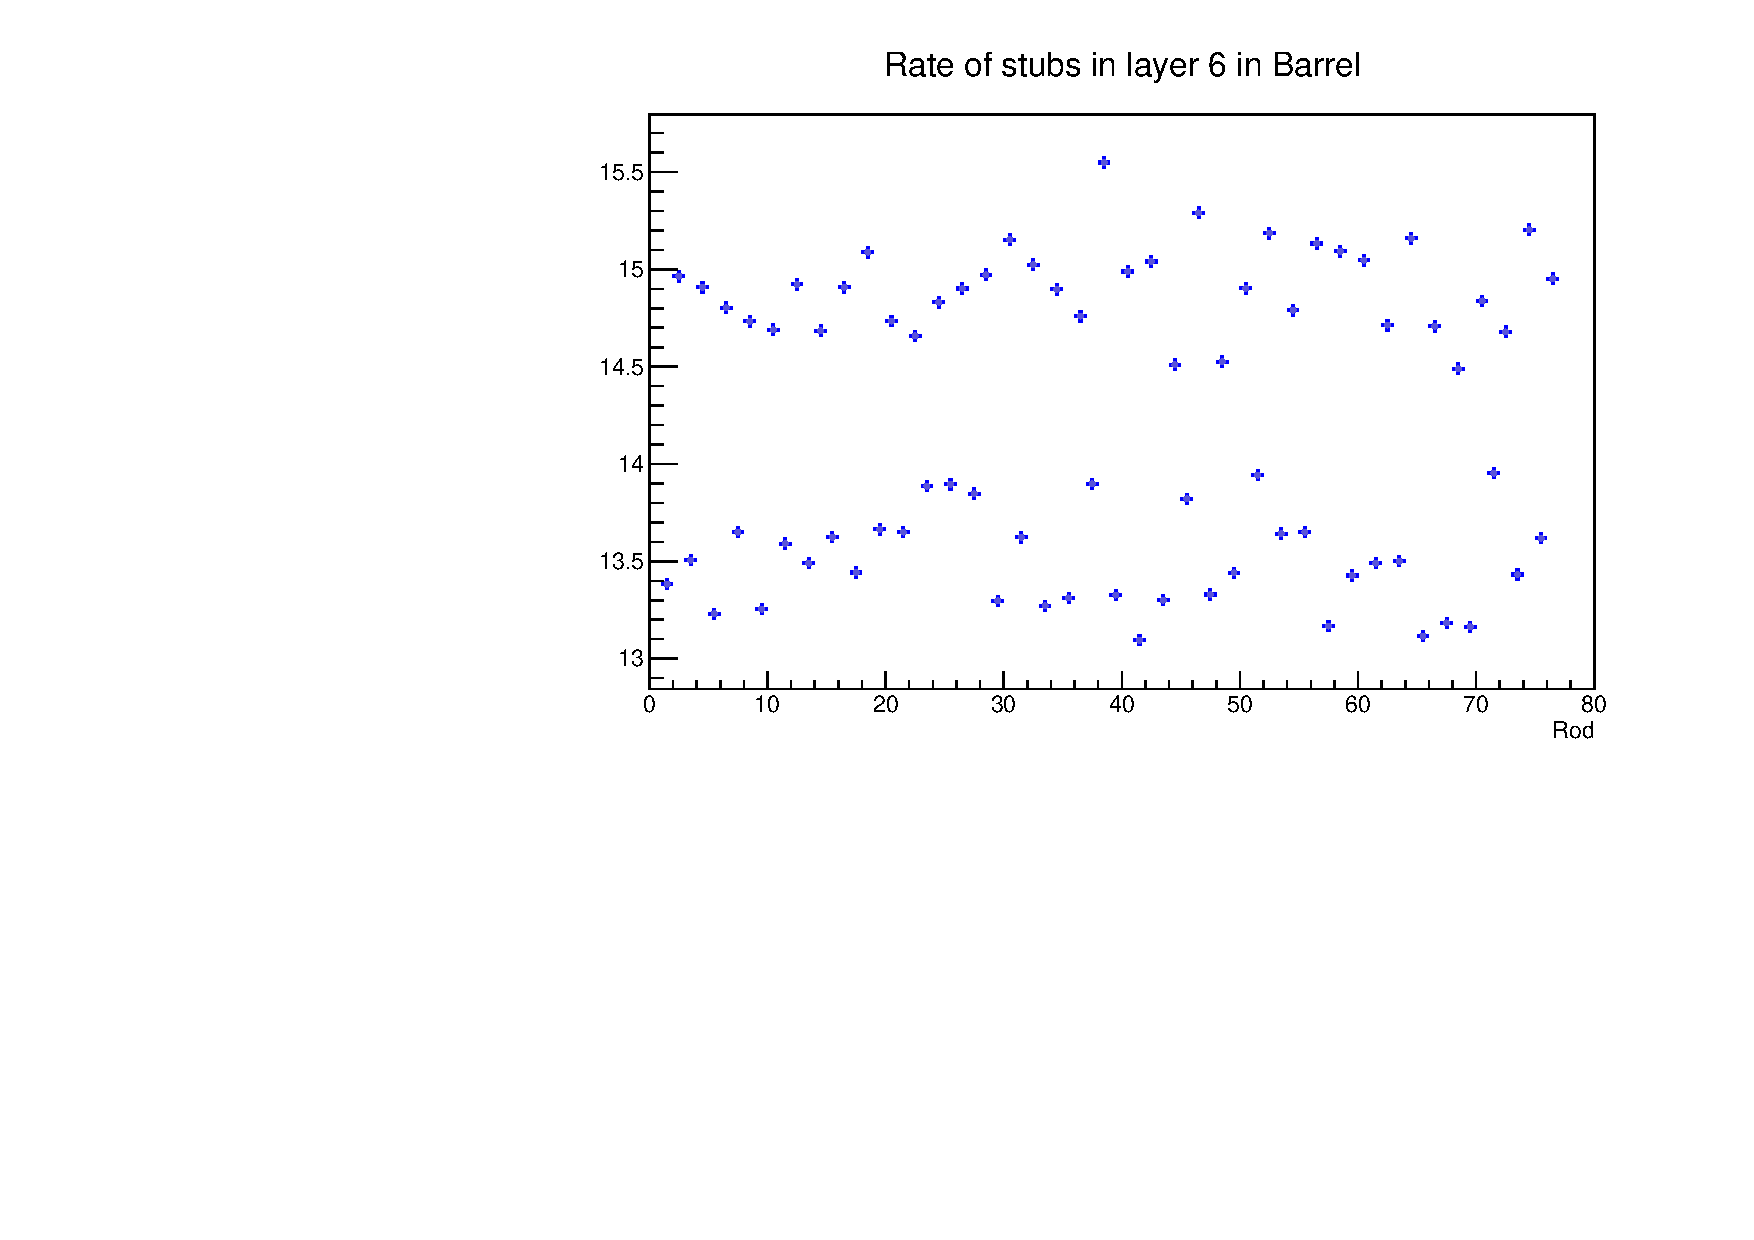
\includegraphics[width=.6\linewidth]{tex/Part2/fig/OT/OT-Rates.pdf}
\caption{
  Average number of track stubs per event per ladder as a function of the ladder id.
  The rate is determined from the CMS Phase II simulation for a pile-up of 200. \nts{PLACEHOLDER: To be replaced with plot using CMS style.}
}
\label{fig:OT_rates}
\end{figure}

